\documentclass[11pt]{article}

\usepackage{hyperref}
\setlength{\oddsidemargin}{0pt}
\setlength{\topmargin}{0pt}
\setlength{\textheight}{8.5in}
\setlength{\textwidth}{6.5in}
\usepackage{graphics}
\usepackage{graphicx}
\usepackage{color}
\usepackage{framed}

\begin{document}
\title{Seven-Letter Word\\Group 1 Final Report}

\author{
	Nipun Arora (nipun@cs.columbia.edu)
 \and Manuel Entrena Casas (mae2135@columbia.edu)
 \and Ben Warfield (bbw2108@columbia.edu)}

\date{December 14, 2009}
\maketitle
\begin{center}
	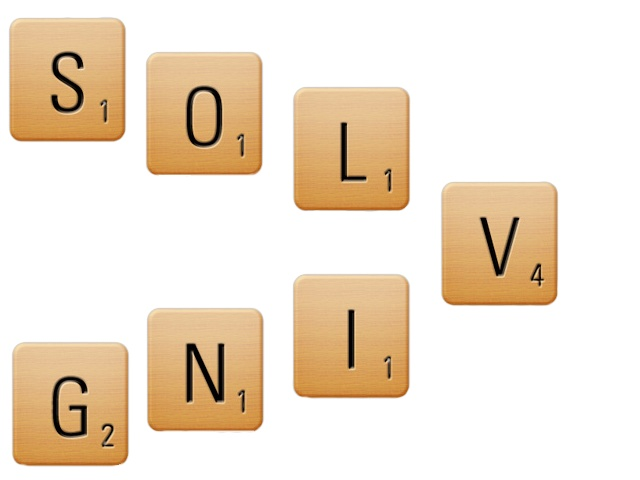
\includegraphics[width=0.7\textwidth]{cover}
\end{center}


\newpage
\setcounter{tocdepth}{2}
\tableofcontents
\newpage

\section{ Introduction }

The aim of the project is to obtain a player that performs as well as possible in a modified version of Scrabble. In this version, the aim is still to form a word with the highest possible score from the letters that we have, but players must bid on the letters to get them, following the rules of the Vickrey auction.

\subsection{Word List}

For a word to be considered valid, it must be included in the provided dictionary. One of the challenges in the project will be searching words efficiently in this list. Therefore, the shorter we can make the list without altering the content, the faster our search for valid words will be. This is accomplished by:

\begin{enumerate}
\item removing words that cannot be formed with the set of letters in Scrabble
\item removing palindromes --words that contain the same letters but in different order
\end{enumerate}

\subsection{Maximizing Seven-Letter Words}

The reward for getting a seven-letter word is 50 points plus the score for each of the letters used in the word, whereas the score for a word with less than seven letters consists only of the sum of the individual letter scores. This means that forming a seven-letter word as often as possible is vital, since the difference in score is very big, and players will not be able to rely on non seven-letter words if they intend to win.

\subsection{Minimizing Costs}

Once it is clear that players must try to get seven-letter words, the next issue will be what cost we are willing to pay for the letters that allow us to form those words. The fact that we have to bid to get letters implies that we might end up forming a seven-letter word and still lose points if we are not careful while bidding so we do not bid more than we will get back. 

On the other hand, other players might use different strategies that force us to be more aggressive in our bidding strategy, so it will be important to balance the amount we bid according to the current situation, and static strategies will clearly be unsuccessful. 

\section{Framework}

There are two main tasks that our player must perform:

\begin{enumerate}
\item infer information from the current situation
\item decide the next action using that information
\end{enumerate}

The player framework that deals with the first task, including data structures and inference algorithms, is explained in the following section, while the tactics used to succeed in getting the necessary letters are explained in the Bidding Strategies section. 

\subsection{Player Architecture}

The basic concept our player architecture revolves around is that the more information we have, the better decisions we can make. Thus, we need to store many diverse facts so we can use that information to decide our next step. These include:

\begin{enumerate}
\item letters we currently have
\item letters that we assume are in the letter bag, thus considered obtainable
\item letters we know other players have
\item our current score and other players score
\item how much we have bid so far in the current round
\item how much all players have been bidding in the current round, as well as in past rounds
\item which words we can reach with the letters we have and the ones that are left in the bag
\item probability of reaching a word, based on the required letters for it
\end{enumerate}

\subsubsection{Operations with Words}

While studying all the information we had we needed to perform many operations with words, abstracting the concept of a word and the operations that it supports. We created a Word class that allowed us to:

\begin{enumerate}
\item access score, length, and letter distribution for a given word
\item check if a word can still be formed with the letters we have
\item find out which letters allow us to go from one word to another
\item calculate the draw probability for a word based on the letters left in the bag and the ones we have
\end{enumerate}

\subsection{A Priori Algorithm} % BEN

As our primary data structure, we chose a data-mining approach using the {\it a priori} algorithm originated by Rakesh Agrawal and Ramakrishnan Srikant (R. Agrawal and R. Srikant.  ``Fast Algorithms for Mining Assocation Rules.''  {\it Proceedings of the 20th VLDB Conference}.  Santiago, Chile, 1994.)  The basic properties of association rules seemed to map well onto the word-building problem space: just as the set of transactions that supports the association of a given pair of items is the intersection of the sets of transactions that include each of them individually,
 the set of words that include any two distinct letters is the intersection of the sets of words that include each of them individually.

\subsubsection{Original Implementation}

Our base implementation was written by Ben Warfield and Ashish Tomar for COMS E6111 (Professor Gravano) in Spring semester of 2009.  It was built to handle a potentially very large number of items (on the order of thousands), grouped in a moderately large set of transactions (less than 18,000 total), and included a number of performance optimizations specific to those parameters, most of which do not apply to the situation where 26 items (the letters of the alphabet) are grouped in 54,000 transactions (the words in the minimized dictionary list).  The basic architecture, however, is equally applicable to both cases: each {\tt ItemSet} object contains a sorted list of transaction IDs (indexes into the word list, in the adapted case), allowing the intersection of two transaction sets to be calculated based on a single parallel pass through the transaction lists of the two {\tt ItemSet} objects.



\subsubsection{Modifications for Word Context}

As mentioned above, the {\it a priori} data structure required several minor modifications before it could be used with the dictionary for this project.  More importantly, however, the algorithm itself has one major incompatibility with the goals of this project: it treats all transactions as sets, ignoring duplication.  Since the set of words containing the letter-set ``Y Y'' is markedly different from the set containing merely ``Y'', this must obviously be corrected.  In an attempt at avoiding jargon collisions, the following discussion will refer to the modified (multiset) item-sets used by the modified algorithm as ``letter-sets,'' and their transaction-lists as ``word-lists.''  

In each round of  the {\it a priori} algorithm, we would normally build new item-sets by intersecting pairs of item-sets from the previous round 
that differ only in their final item (sorted canonically)--so if we have item-sets ``A B'' and ``A C'', we can intersect them to form a new set ``A B C,''  which has as its transaction-list the intersection of the transaction-lists from ``A B'' and ``A C.''  Thus far, the algorithm translates perfectly to the letter-set/word-list situation: letter-sets ``A B'' and ``A C'' can be used to form ``A B C,'' whose word-list should be the intersection of the word-lists of the two parents.  Unfortunately, the original algorithm (since it ignores duplication) explicitly avoids building a new item-set based on two identical item-sets from the previous round:
if we attempt use the unmodified algorithm on letter-sets ``A B'' and ``A B'', we will obtain a letter-set labeled ``A B B'' whose word-list actually contains all of the words from ``A B'' (since the intersection of a set with itself is the original set)--a dramatically incorrect result.

The solution we chose for this problem is a simple special-case: each time we wish to intersect an item-set with itself, we first determine the letter of interest (always the last letter in the item-list) and the number of times it repeats in the current item-list, then
retrieve the actual words represented by the item-set's transaction IDs, and count the number of occurrences of the duplicated letter in each word.  Words containing strictly more copies of the letter of interest than are in the current item-list are retained for the ``intersected'' item-set, while others are dropped.  A more efficient implementation would cache this information (presumably using the {\tt Word} objects already required by the player), but since the entire execution time of the modified algorithm on our wordlist is under 10 seconds, this was not judged worth the effort.

\subsection{Unreachable Words}

Each time a letter is picked up by another player, some words become impossible for our player to reach, no matter which tiles are available in the remaining auctions.  The data-mine structure (once letter repetition is allowed) actually provides a very easy way to find these words: any word that would require all the copies of this letter that are already in our rack, and all of the copies of this letter that were \textit{previously} in the letter bag, is now unreachable.  More explicitly, to find the newly-unreachable words, we must
\begin{enumerate}
\item find the number of copies of this letter that were in the letter bag before this tile was drawn (which may any where from 1 to 12)
\item find the number of copies of this letter that we have in our own rack
\item take the sum of these two numbers, and query the data mine for all words that include that number of this letter.
% that's kind of incoherent, Ben
\item if there are any such words, add them to our set of ``unreachable'' words.
\end{enumerate}

This technique will generally result in some words being marked as ``unreachable'' multiple times, but since the transition from reachable to unreachable is one-way, and the state maintenance is cheap (a simple array of booleans, indexed by word ID), the redundancy is of minimal concern.

\subsection{Probability Calculations} %BEN 

We can readily generate, at any time, the list of seven-letter words that we could reach this round.  However, at the beginning of a round, this list will contain both ``zymurgy'' and ``euchres,'' which are clearly not equally probable words for us to reach by the end of the round.

Obviously, we need some way to judge the relative ease of reaching each of the possible seven-letter words.  Ideally, this should be easy to recalculate as the letter distribution in the bag and on our rack shifts over the course of the round.


\subsubsection{Naive Sequence Probability Approach}

As a first approximation, we can trivially calculate the probability of any specific letter being drawn from the letter bag on the current turn.  By taking the product of this probability for all remaining letters in a word, we can easily calculate an approximation of the probability of that word being reached.  This calculation has several disadvantages: most obviously, it ignores the changing denominator of the probability calculation as letters are drawn, as well as the changing numerator for repeated letters.  It also takes no account of the fact that other letters may be drawn between the ones we are interested in.  To balance the first disadvantage, it has the advantage of being very simple and fast to calculate for many words; for the second, we observe that the impact of this effect is roughly the same for all words, so we should still be able to use this value to compare different words, since both will be wrong in the same way.

\subsubsection{Sequence-Counting Approach}
\label{sec:sequenceCounting}

The principal defect of the naive approach is that it fails to take account of the effects of drawing without replacement.  This can be addressed by making the calculations somewhat more complicated.
% XXX genius prose there...

For a given configuration of the letter-bag and our own rack, we can calculate the number of possible draw sequences that would lead to a given word using fairly simple combinatorics--simple, at least, if we consider only draws that are relevant to the word itself.  For each a letter index $i$ between 1 (``A'') and 26 (``Z''), let $w_{i}$ be the number of appearances of that letter in a given word, $b_{i}$ be the number of copies of that letter remaining in the bag (or at least, potentially remaining there), and $r_{i}$ be the number of copies of that letter that we currently have on our rack.  Then the number of possible draw sequences that can lead to our being able to form this word is

% good thing we're not using Google, after all...
$$\prod_{i=1}^{26}{b_{i}\choose w_{i} - r_{i}}*\left( \sum_{i}w_{i} - r_{i}\right)!$$

The probability of our seeing a specific collection of letters over the course of the remaining letter auctions could in principle be calculated beginning from this expression: we attempted this calculation, but realized while doing so that once again, the actual probability was less important than the relative weights of the different words.  Moreover, the actual probability of a set of letters appearing is in any case an upper bound on the likelihood of our forming that word, since we might be outbid for any or all of the letters in question.  Accordingly, we made the sequence-count, rather than an actual probability, the basis for all of our later probability-based calculations.  (Note that this renders the factorial at the end of the above expression useless: since all reachable seven-letter words will always have draw sequences involving the same number of letters, this term will effectively be constant.)

The failure to finish this probability calculation does have one important consequence: since we omit the portion of the probability calculation that depends on the total number of draws from the letter-bag, the count for a given word remains unchanged until and unless one of the letters in it is drawn from the bag.  This allows us to avoid expensive recalculations: if we precalculate the sequence counts for each word for the starting position (an empty rack and a full letter-bag), only a relatively small number of words (those including the letter that was bid on during the previous turn) must be recalculated each turn.

There are two important caveats to note, however:
\begin{enumerate}
\item there is no explicit accounting in this calculation for the hidden letters that may already be in other players' racks: since we have no way of knowing (and we make no attempt to guess) what these letters are, their only impact on the game is to reduce the total number of draws from the bag.
\item however, as noted previously, we take no account of the number of letters remaining to be drawn.  Since the probability of a given collection of letters being drawn is clearly higher when there are many turns left in the round than when there are few turns remaining (all other things being equal), this is a serious defect.  Considering the complication involved in the explicit probability calculation, however, we decided to leave this problem aside for later consideration.
\end{enumerate}



\section{Bidding Strategies}

\subsection{When to Bid}

Our high-level bidding strategy is simple: we query the {\it a priori}-generated data mine using the set of letters we have in our rack at the moment, and determine what (if any) seven-letter words include them.  If any of these seven-letter words remains reachable (no matter how unlikely the possibility), we will bid only on letters that help us reach one of those words.
If no such word exists, we simply bid incrementally: we find the best-scoring word we can make with our existing rack and the best-scoring word we could make if we acquired the letter currently up for bid, then bid the difference (if positive) between the two scores.  This strategy, much discussed in class, has a worst-case behavior of zero gain, and (in contrast to any strategy that takes into account what other non-seven-letter words we might hypothetically form with other letters) is extremely simple to implement.

\subsection{Gain-based strategies}

Our initial approach to bidding (once we gave up on the ``bid 0 and make the best of it'' strategy) attempted to bid based on how much closer acquiring a particular letter would bring us to having a seven-letter word.  

Assuming that we can reach a seven-letter word after getting the current letter, our final score would be 50 plus the sum of the score of all the letters we use. According to the rules of the Vickrey auction, if we bid what we are willing to pay, we will not be paying more than this amount in the event we win the bid, but we might pay less. Combining these two facts, our idea was to bid an amount such that the total amount we bid after getting all seven letters is not greater than the value of the seven-letter word we will get. Let $c$ be the cumulative amount we have paid thus far, $s$ the score for the offered letter, and $n$ the number of letters we have, then we would bid:

$$\frac{50+s-c}{7-n}$$

This strategy is intuitively reasonable: if we succeed in every bid, we will have paid a cost no higher than the benefit (50 points + letter scores) that we expect from forming a seven-letter word.

\subsubsection{Word Count}

Just allowing us to reach a seven-letter word does not mean that the current letter is necessarily a good acquisition. The amount of seven-letter words that can be formed after getting that letter might be ridiculously small, so we must have some way to determine not only if a letter is good for us, but more importantly how good it is. Our first approach used the number of reachable words after acquiring the letter, as compared to the total number of reachable words before acquiring it. Generally speaking, the first number will be smaller than the second, but the fraction they form will give us an estimation of how good the letter is.

After calculating this fraction, we checked if it was greater than a given cutoff, obtained after several empirical tests, and if the value was greater than the cutoff, then we would go ahead and bid for the letter. For example, if the cutoff was 0.3, int the case we could reach 1000 seven-letter words with the letters we have, and 400 after we get the offered letter, we would bid for the letter. If we could only get 200 after getting the letter, then we would not bid. 

If $t$ is the number of currently reachable seven-letter words, $r$ is the number of reachable words after getting the letter, and $c$ is the cutoff, we would only bid for the letter if

$$\frac{r}{t}>c$$

\subsubsection{Summed Word Probabilities}

The next step was to polish our strategy by using more significant information. The number of words reachable from the set of letters we have does not take into consideration the combined probability of those words being reached. It might be possible that many of them were reachable only by means of an infrequent letter, and this should affect our estimation of how good an offered letter is for us.

By using the probability of each individual letter in the bag of letters, we can calculate the probability of a word being formed. 
The measure we will use then is the summed probability for all reachable seven-letter words after acquiring the offered letter, and we will compare this value to a cutoff, as before. This resulted in a more accurate estimation of how convenient bidding on a letter is.

As an alternative approach, we used these summed probabilities to rank all of the letters remaining in the bag, with an eye toward selecting only letters from the upper end of this ranking: for letters with very high ranks, we would bid large amounts; for those with medium ranks, small amounts; for those with low ranks, nothing.  Unfortunately, once we implemented this approach we realized a major drawback: we might pass over medium-ranked letters, then choose a high-ranked letter that required one or more of those medium-ranked letters to actually form a seven-letter word.

\subsubsection{Summed Word Draw Possibilities}

Our next alternative used the letter-sequence-counting approach outlined in section \ref{sec:sequenceCounting}: given the number of sequence possibilities that would allow us to reach a seven-letter word from our current position, how many of them involve at least one copy of the current letter?  Assuming the cached letter-sequence-counts are kept up to date as outlined above, this is trivial to implement: we simply find the set of seven-letter words that include our current letters plus the letter being bid on, sum their sequence counts, and compare that quantity to the sum of the sequence-counts for seven-letter words reachable from our current rack without the added letter.

From this, we can again resort to a heuristic cutoff value to decide which letters we do and do not wish to bid on.  For the bidding strategy based on this calculation, we used an initial cutoff of $0.4$ (based purely on our observations of the range of values we were seeing during testing): any letter which allowed us to retain more than 40\% of our possible routes to a 7-letter word was worth bidding on.  To guard against excessive conservatism, we  dropped this cutoff to  $0$ (that is, any non-zero retained fraction) any time the number of auctions remaining in this round dropped below twice the number of letters we still needed to acquire.

\subsubsection{Summary}

These strategies successfully rescued our player from stinginess, allowing us to form seven-letter words with increasing frequency.  The cost they imposed, however, was disproportionate to the benefit: our player generally averaged significantly positive scores, but would fall far behind those of other groups.

\subsection{Loss-based strategies}

The obvious alternative to gain-based bidding is loss-based bidding: each time a letter is placed up for bid, we estimate how badly our chances of reaching a 7-letter word would be hurt by not acquiring it, then multiply that penalty by the benefit we would forgo (again, 50 points).  

\subsubsection{Basic Calculation}

This is done by checking, for every reachable seven-letter word, how the probability of reaching it is affected if we remove the offered letter from the bag. These differences are added, and this result divided by the total sum of probabilities for reachable word to give us a measure of how our chances to get to a seven letter-word would be reduced if we let go this letter. Let $p_i$ be the current probability of word i, $n_i$ the new probability if we remove the offered letter from the bag, and $R$ the set of all currently reachable seven-letter words, then we will bid:

$$\frac{\sum_{i \in R}p_i - n_i}{\sum_{i \in R}p_i} * 50$$

\subsubsection{Opportunity Cost}

This strategy brings us back face to face with the problem we declined to solve earlier: how does the probability of a given sequence of letters being reached change with the number of remaining auctions?  Clearly, we lose some probability of reaching a seven letter word with the passage of each turn, regardless of the letter seen, but we do not yet have a good way of calculating that loss.  From the beginning, our player tracked the number of total auctions in the round, and the number that had already taken place, so we would be able to alter our bidding based on the time remaining.
As the round draws closer to its end, we want to get our seven letter words before the remaining auctions are so few that we end up having to take letters we do not want, but how much of our opportunity to reach a seven-letter word do we lose each time a round goes by without our collecting a letter? 

Our earlier players tracked the value of $\frac{auctions\_left}{letters\_needed}$, and simply escalated the bid (or increased the number of letters we were willing to bid on) if this value became too low, but this was a very crude and unsatisfying heuristic.  The initial loss-based bidding strategy instead multiplied all of its bids by $1+\frac{1}{auctions\_left}$, so we would bid higher as the round progressed (assuming any letters worth bidding on were drawn) .  This was moderately effective, if 
still unsatisfactory.  Unfortunately, our subsequent efforts to improve on this heuristic were unsuccessful--our final player still uses this multiplier. 

\subsubsection{Market Rates}

In principle, if we are able to form a perfect estimate of the opportunity cost of passing on one auction, as well as the penalty for failing to acquire each letter, we should be able to perfectly calculate the value (in expectation) of each letter, and our player should perform well, at least on average.  However, since our estimates are (as discussed in the previous section) imperfect, and we may be in competition with other players, we also attempt to keep track of how our bids compare to the ``market rate'' for each letter: if we are losing out on our bids consistently, we may be systematically underestimating the value of letters.

We considered a number of tactics for adjusting our bidding to avoid falling behind on letter acquisition:

\begin{enumerate}
\item{} periodically boosting our bid by some fixed amount or factor, to avoid consistently being outbid (and confound any opposing-team predictors)
\item{} keeping track of the number of letters acquired and the number of bidding rounds, and boosting our bid if we are behind the ``average'' rate of letter acquisition (that is, if more than $1/7$ of letters have been auctioned off, but we have only 1 or 0 letters on our rack). % shouldn't it be 1/no_players ?
\item monitoring our success rate on recent bids, and boosting the bid by a fixed factor if we have been losing bidders some number of times in a row
\item extending the previous strategy by maintaining (or continuing to escalate) the boost factor until we succeed on a bid.
\item keeping track of the bidding statistics (average and standard deviation) to ensure that our bid is not too far from the average bid value, preventing under-bidding and over-bidding
\end{enumerate}

We evaluated all of these approaches in mini-tournaments, against each other and the most recent version of players from the other groups: our final conclusion was that the penalty for underbidding was not crippling us in any case, so a relatively conservative modification to our bidding would suffice.  Our final player tracks the success or failure of each non-zero bid, and boosts its bids by a factor of 2 if the last three or more non-zero bids have been unsuccessful. %again, maybe we should have used no_players instead of 3



\section{Tournament Results} % NIPUN
	Our G1Player seems to do pretty well in almost all tournaments, ranking amongst the top teams on an average. We especially do well in tournaments with more opportunities to score seven letter words (i.e. more no of players). Overall we also seem to have form a high no of seven letter words. On the other hand relative to other tournaments our performance in tournaments with lesser no of players is not as good. This basically shows that given a good chance of forming seven letter words, we are generally the most successful amongst the given teams and do well in terms of the score.
	
	To give a high level view of our performance in relation to other players we look at the 1 player each tournament, and 2 instances of each player tournament. Since they have all the players these two give a good idea of the performance of a player with respect to others. 
	
	\subsection{Performance in terms of Score}
	
	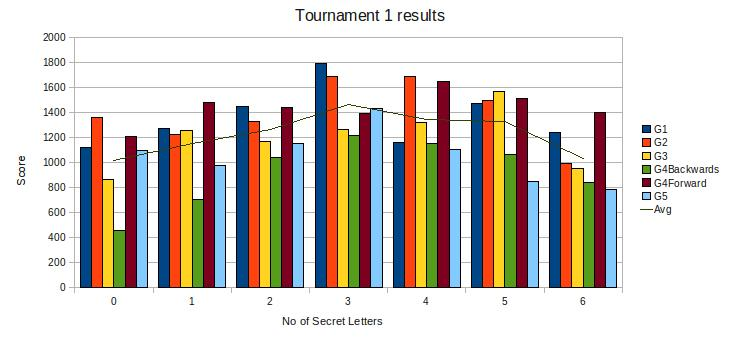
\includegraphics[width=1\textwidth]{T1Results}
	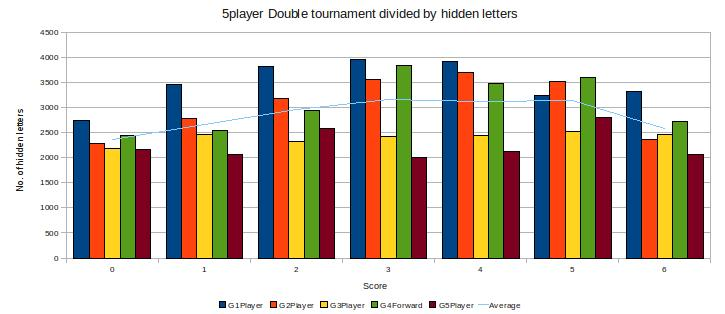
\includegraphics[width=1\textwidth]{T2Results}
	
	Our performance in Tournament 1 where there was only 1 instance of each player, was really good, and it can be clearly seen that G1,G2 and G4Forward player are the candidates for the top slot. However, we outperform all teams in tournament 2 where there are 2 instances of each player hence a lot more opportunities to fom seven letter words. We observed that this behaviour was consistent in all tournament results and in some test cases we ran ourselves. We attribute our relatively poor behaviour in tournaments with lesser no of players to the fact that we did not properly account for the no of players in our bidding strategy. However, we still remain competitive in cases where there are less no of players.
	
	\subsection{Performance in terms of No. of Seven Letters}
	
	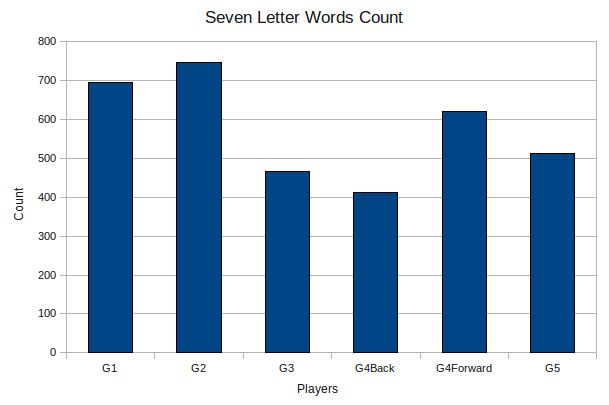
\includegraphics[width=0.8\textwidth]{SevenCount}
	
	While seven letter words are not the actual parameter of success, they are a huge contributing factor. We found that a high seven letter word count usually converted into a higher score for a player. Once again team 1 and team 2 are the top teams in forming the seven letter word. While we beat team 2 beats us in the no of seven letter words formed we beat them in the overall score at the end of the tournament.(Team 1 Cumulative Score: 33272, Team 2 Cumulative Score: 30461). We explain the significance of this statistic in the next section.
	
	\subsection{Avg Bid Per Letter/ A deeper look}
	To further understand the results we look at avg amount paid by each player in the case when they form a seven letter word and in the case when they do not form a seven letter word. The source for both these tables were the first two tournaments. 
	\begin{center}
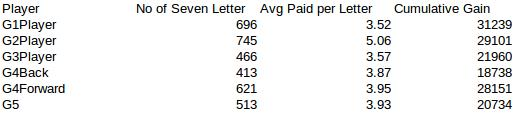
\includegraphics[width=0.8 \textwidth]{AVGBidSevenY}
\end{center}
The table above shows the avg amount paid per letter by each team, the no of seven letter words formed by them and their cumulative gain for all rounds where they do return a valid seven letter word.(It would have been interesting to see the actual bids, however we can say intutively that on an average the bid amounts by each player is proportional to the amount they paid for it). Clearly G2 pays the highest for forming seven letter words and makes the maximum seven letter words. However, in terms of pure numbers we over take them with a relatively high no of seven letters and lesser avg pay per letter. 
	\begin{center}
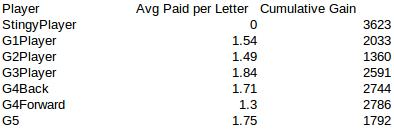
\includegraphics[width=0.6 \textwidth]{AVGBidSevenN}
\end{center}
	Clearly the biggest contributing factor to the score is the 50 point bonus the player gets on returning a seven letter word. However, non-seven letter words also cumulatively addup to the score and produce a significant difference. In the above table we show the avg gain per round ((No of points gained- amount bid) per round) of each team when not forming a seven letter word. While we i.e. team 1 seem to do reasonably well. Team 4 seems to manage situations where seven letter word is not formed much better than us, this could be a contributing factor towards their success in the tournament. On the other hand team 2 seems to be the most heavily penalized in the non seven letter word formin scenario as it pays the most and gains the least. 
	\subsection{Head to Head Analysis}
	There were two kinds of head to head tournaments played , the first being 1 vs 1 where there was 1 instance of 2 players, and the other being 5 v 5 where there were 5 instances of each player. 

\subsubsection{1v1 tournaments}	
	In the 1 v 1 tournament our performance was relatively bad which again we base on the fact that there were too few chances of making a seven letter word, and because of a little overbidding on our part we get penalized in such cases. In the 1v1 tournament we beat only player g3 and in a few instances do better than other players with a high no of hidden letters. We do not dig deep in 1v1 tournament results as there is a large variability in cases with high no of hidden letters( 5 or 6) and only 2 competing players. 
	\subsubsection{5v5 tournaments}
	In the 5v5 tournament we beat most players convincingly and only g2 and g4 give us a run for the money. For the sake of brevity we discuss our relative performance with them in the charts shown below.\\
	\textbf{G1 vs G2}\\
	The graph below shows seven letter word counts for G1 and G2 as well as the average gain per round for all the 5 instances of each player put together(i.e. cumulative scores/50). While G2 generally makes more seven letter words than us, they seem to overpay for their letters by quite a margin, which enables us to beat them in nearly all instances(except for 6 hidden letter where the chance of forming a seven letter word is less). This basically shows that g2 in general bids more than us and is hence able to form seven letter words frequently. However we make them pay heavily for it :).
	\begin{center}
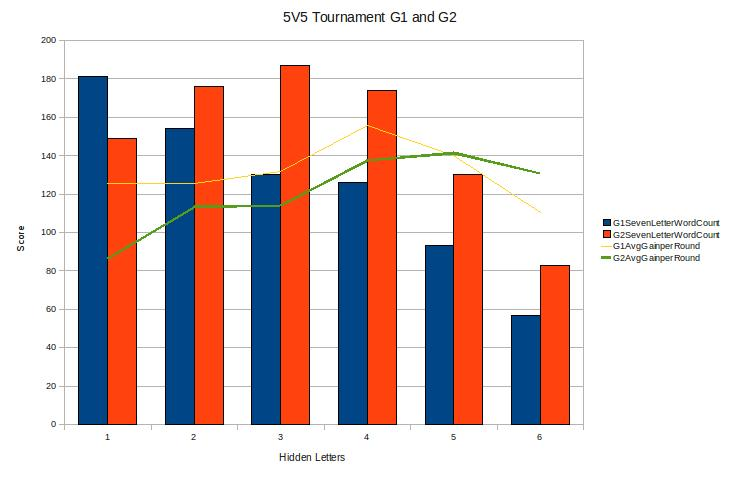
\includegraphics[width=1 \textwidth]{5v5option3G1G2}
\end{center}
	\textbf{G1 vs G4 Forward}
	The graph for G1 vs G4 is much more proportional to the amount of words formed. However an important feature in this graph and the earlier one is that both g2 and g4 seem to do better as the no of hidden letters increase. While we generally beat them when there are less hidden letters, this basically means that we are better than them at finding pathways to a seven letter word. However in higher no of hidden letter case, they probably bid higher and are able to grab letters before us.
	\begin{center}
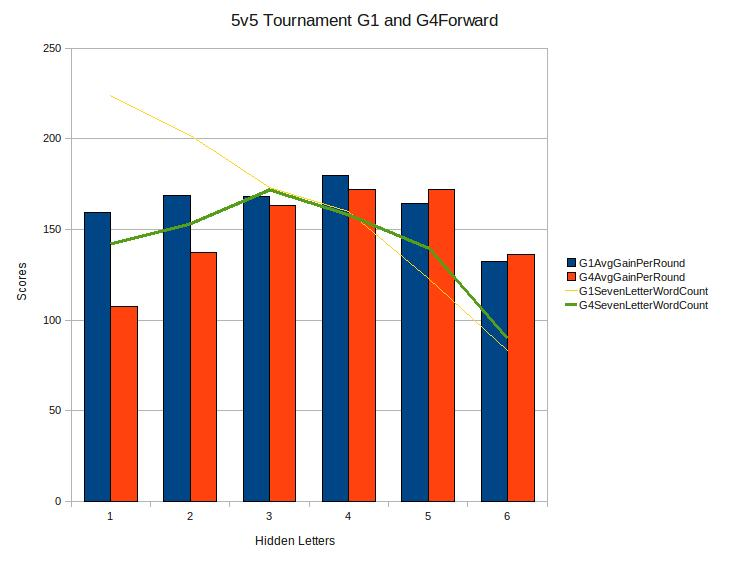
\includegraphics[width=1 \textwidth]{5v5optionG1G4}
\end{center}
	\subsection{Competing against ourselves vs Competing with others}	
	We do really well in competing against ourselves compared to other players, we beat all others by a considerable margin. This is also shown in our high word count. 	
\begin{center}
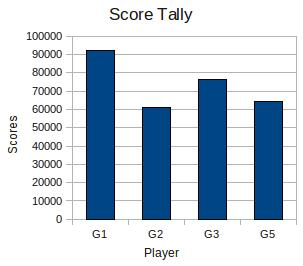
\includegraphics[width=0.5 \textwidth]{AllPlayerScoreTally}
	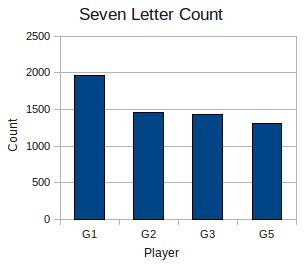
\includegraphics[width=0.5 \textwidth]{AllplayerWordCount}
\end{center}
However, in general most teams pay more per letter in comparison to other tournaments where they are not competing against themselves. This can basically be attributed to the fact that they have similar bidding strategies and they basically compete for the same letter bidding in the same range hence on an average increasing the amount they pay for the letter. 
\begin{center}
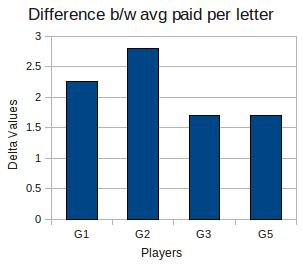
\includegraphics[width=0.5 \textwidth]{ALLPlayer}
\end{center}

In particular team 2 pays heavily for each letter in the all same player tournament, but is forming comparitively less seven letter words (i.e. team 2 in particular seems to harm itself the most resulting in a bad performance overall in the all player tournament)
	\subsection{Summarizing Tournament Analysis}
		
	Digging deeper into the tournament statistics we discovered that success in the tournament can basically be attributed to two factors:
	--Insert Graphs
	\begin{enumerate}
	\item{} A relatively high bid per letter: This seems most likely as bidding values are most likely proportional to paid values and the teams which have paid higher for their letters have generally done well. Overbidding however in some cases seems to have adversely effected to an extent(team 2, and team 1 in 1v1 tournament)
	\item{} A good letter evaluation strategy: Teams which have done well also seem to bid low for letters which do not form a seven letter word, and seem to be properly able to evaluate the worthiness of a letter to them(as they have a high seven letter count as well)
\end{enumerate}



\section{Possible Extensions}

As is perhaps clear from the foregoing discussion, the single largest improvement we could make to our player if we developed it further would be to give it a more explicit (and theoretically sound) calculation for the change in word probabilities over the course of each round.  Our existing heuristics are useful, and sufficient in many circumstances, but correctly calculating this value might well have enabled our player to sweep the tournaments.

Another thing we would have liked to do (or to make more use of, to the extent that we did implement it in this player) was to keep track of other players, trying to predict their next move by studying their previous behavior, and having a representation as accurate as possible of their status. It would have given us better control over the game flow.

Finally, it would be interesting to have more explicit probability calculations for the (admittedly rare) late-game situation where the player must decide between bidding on a profitable increment (say, a Q that would boost us from 5 to 15 points, but rule out any possible seven-letter words) and holding out for an unlikely seven-letter word. Given the fact that other players may still be bidding, and we may not know exactly which letters remain in the bag, it may not be possible to obtain the precise probability of getting the letters we need to complete the seven-letter word, but it should be possible to set an upper bound on it, which would let us determine if the increment is worth more to us than the value in expectation of trying for the 50-point bonus.  Given how rarely this event occurs, and how small the score improvement is likely to be, however, this would be a low-priority enhancement.



\section{Acknowledgements}

Thanks are due to Jonathan Bell for the anagram-filtered word-list (which brought the size of the dictionary down from over 70,000 to under 55,000).  We also made heavy use of the MySQL database he made available to the class for our analysis section.

Thanks are clearly also owed to Professor Gravano for assigning the Agrawal {\it a priori} paper and its implementation for COMS E6111 last spring, and to Dr. Virginia Warfield, Ph.D., for getting Ben interested in probability, about 20 years ago.

\section{Contributions}
General strategies were discussed by the group as a whole, and the final experimental comparison of players was done as a group.  Specific code contributions were as follow.

Ben adapted the {\it a priori} code from his previous homework to be useable for this assignment, as well as writing the combinatorics code and the initial (extremely simple) loss-based bidder.

Manuel wrote lots of bidding strategies and I'm totally asleep right now

Nipun did the tournament analysis, made the initial player/probability calculation , subset checking for word formation and the initial percentile bidding strategy

\section{Issues Encountered and Conclusions}

The great amount and complexity of data structures needed to obtain a satisfactory solution to our expectations for this project made it hard to keep track of all the different changes, bugs, and bottlenecks. The draw-sequences code (section \ref{sec:sequenceCounting}) had a bug early on which may have compromised some of the comparisons we made, which we did not successfully diagnose for some time.  We are confident we ended up with a good solution, but the path we took to it was definitely not always smooth.

Moreover, we soon learned that one strategy alone (at least, of the strategies we were able to develop) is not good enough, and taking other players' strategies into consideration while designing our own strategy is necessary. A player performs well while its strategy is adequate in relation to its opponents and the type of game: strategies that appeared promising in large-scale matches with few hidden letters performed extremely poorly in matches with fewer bidding turns, and inversely.

In the end, when all of the different strategies from different players and the implications of the Vickrey auction are taken into account, the fundamental question asked by this project is ``what is the value of a letter?''  If it were still September, this question could provoke either an interesting philosophical debate or an extended dive into the the twistier weeds of probability theory.  At this point in the semester, however, we are happy to have found a reasonably successful heuristic calculation to solve this final problem.

\end{document}
